
%(BEGIN_QUESTION)
% Copyright 2005, Tony R. Kuphaldt, released under the Creative Commons Attribution License (v 1.0)
% This means you may do almost anything with this work of mine, so long as you give me proper credit

Potentiometers are very useful devices in the field of robotics, because they allow us to represent the position of a machine part in terms of a voltage.  In this particular case, a potentiometer mechanically linked to the joint of a robotic arm represents that arm's angular position by outputting a corresponding voltage signal:

$$\includegraphics[width=15.5cm]{i01513x01.eps}$$

As the robotic arm rotates up and down, the potentiometer wire moves along the resistive strip inside, producing a voltage directly proportional to the arm's position.  A voltmeter connected between the potentiometer wiper and ground will then indicate arm position.  A computer with an analog input port connected to the same points will be able to measure, record, and (if also connected to the arm's motor drive circuits) control the arm's position.

\vskip 10pt

If we connect the potentiometer's output to a {\it differentiator} circuit, we will obtain another signal representing something else about the robotic arm's action.  What physical variable does the differentiator output signal represent?

$$\includegraphics[width=15.5cm]{i01513x02.eps}$$

\vskip 20pt \vbox{\hrule \hbox{\strut \vrule{} {\bf Suggestions for Socratic discussion} \vrule} \hrule}

\begin{itemize}
\item{} Sketch an operational amplifier circuit capable of performing this differentiation on the position signal.
\item{} What physical variable would we be calculating if we differentiated the output of the first differentiator circuit?
\end{itemize}

\underbar{file i01513}
%(END_QUESTION)





%(BEGIN_ANSWER)

The differentiator circuit's output signal represents the angular {\it velocity} of the robotic arm, according to the following equation:

$$\omega = {d\theta \over dt}$$

\noindent
Where,

$\omega$ = angular velocity, in degrees or radians

$\theta$ = angular position, in degrees/second or radians/second

$t$ = time, in seconds

%(END_ANSWER)





%(BEGIN_NOTES)

This question asks students to relate the concept of time-differentiation to physical motion, as well as giving them a very practical example of how a passive differentiator circuit could be used.  In reality, one must be very careful to use differentiator circuits for real-world signals because differentiators tend to amplify high-frequency noise.  Since real-world signals are often ``noisy,'' this leads to a lot of noise in the differentiated signals.

\vskip 10pt

If we differentiate the signal again with respect to time, we get angular acceleration:

$$\alpha = {d\omega \over dt} = {d^2 \theta \over dt^2}$$

%INDEX% Mathematics, calculus: derivative (applied to robotic arm position)
%INDEX% Process: robot welder

%(END_NOTES)


